\documentclass{article}
\usepackage{amsmath, amssymb, graphicx, tikz, pgfplots, booktabs, xcolor}
\pgfplotsset{compat=1.18}

% Custom environments as requested
\newenvironment{lesson-meta}{}{}
\newenvironment{item-analysis}{}{}
\newenvironment{model-discuss}{}{}
\newenvironment{concept-box}{}{}
\newenvironment{concept-summary}{}{}
\newenvironment{example}[1]{\textbf{Example #1}\par}{\vspace{1em}}
\newenvironment{tryit}[1]{\textbf{Try It! #1}\par}{\vspace{1em}}
\newenvironment{practice}[2]{\textbf{#1.}}{\vspace{1em}}
\newenvironment{te-addendum}[2]{}{}

% Custom commands
\newcommand{\answer}[1]{\par\textbf{Answer:} #1}
\newcommand{\placeholder}[2]{[\textit{#1: #2}]}
\newcommand{\uncertain}[2]{#1}
\newcommand{\te}[1]{}

\begin{document}

\begin{lesson-meta}
\textbf{4-5 Solving Rational Equations}

\textbf{I CAN...} solve rational equations and identify extraneous solutions.

\textbf{VOCABULARY}
\begin{itemize}
    \item rational equation
    \item extraneous solution
\end{itemize}

\textbf{ESSENTIAL QUESTION}
How can you solve rational equations and identify extraneous solutions?
\end{lesson-meta}

\begin{model-discuss}
\textbf{CRITIQUE \& EXPLAIN}

Nicky and Tavon used different methods to solve the equation $\frac{1}{2}x + \frac{2}{5} = \frac{9}{10}$.

\begin{center}
\begin{tabular}{cc}
\textbf{Nicky} & \textbf{Tavon} \\
$\frac{1}{2}x + \frac{2}{5} = \frac{9}{10}$ & $\frac{1}{2}x + \frac{2}{5} = \frac{9}{10}$ \\[6pt]
$\frac{1}{2}x = \frac{9}{10} - \frac{2}{5}$ & $10\left(\frac{1}{2}x + \frac{2}{5} = \frac{9}{10}\right)$ \\[6pt]
$\frac{1}{2}x = \frac{5}{10}$ & $5x + 4 = 9$ \\[6pt]
$x = 1$ & $5x = 5$ \\[6pt]
& $x = 1$ \\[6pt]
The solution is 1. & The solution is 1. \\
\end{tabular}
\end{center}

\textbf{A.} Explain the different strategies that Nicky and Tavon used and the advantages or disadvantages of each.

\textbf{B.} Did Nicky use a correct method to solve the equation? Did Tavon?

\textbf{C. Use Structure} Why might Tavon have chosen to multiply both sides of the equation by 10? Could he have used another number? Explain.
\end{model-discuss}

\begin{concept-box}
\textbf{VOCABULARY}
A \textbf{rational equation} is an equation that contains a rational expression.
\end{concept-box}

\begin{example}{1}
\textbf{Solve a Rational Equation}

What is the solution to each rational equation?

\textbf{A.} $\frac{1}{x+4} = 2$
\begin{align*}
(x+4)\left(\frac{1}{x+4}\right) &= 2(x+4) \\
1 &= 2x + 8 \\
x &= -\frac{7}{2}
\end{align*}
The solution is $x = -\frac{7}{2}$.

\textit{Note: Multiply both sides of the equation by the common denominator to eliminate the fractions. Then solve. Confirm that the solution is valid in the original equation.}

\textbf{B.} $\frac{1}{x-3} = 5$
\begin{align*}
(x-3)\left(\frac{1}{x-3}\right) &= 5(x-3) \\
1 &= 5x - 15 \\
x &= \frac{16}{5}
\end{align*}
The solution is $x = \frac{16}{5}$.
\end{example}

\begin{tryit}{1}
What is the solution to each equation? \\
\textbf{a.} $\frac{2}{x+5} = 4$ \answer{x = -4.5} \\
\textbf{b.} $\frac{1}{x-7} = 2$ \answer{x = 7.5}
\end{tryit}

\begin{example}{2}
\textbf{Solve a Work-Rate Problem}

Arthur and Cheyenne are making Chinese paper cutting designs to give as gifts to wish family and friends good luck in the coming year. Together they can complete the job in 24 hours. How long would it take Cheyenne to complete the job if she was working alone?

\placeholder{illustration}{Arthur and Cheyenne working on Chinese paper cutting designs. A speech bubble from Cheyenne reads: "Cheyenne works twice as fast as Arthur."}

\textbf{Step 1} Determine the work-rates of Arthur and Cheyenne.

Let $x$ represent the number of hours Arthur needs to finish the job himself.
\textit{Note: The amount of a job completed per hour is the work-rate.}

Arthur works at a rate of $\frac{1 \text{ job}}{x \text{ hours}} = \frac{1}{x} \frac{\text{jobs}}{\text{hour}}$.

Cheyenne is twice as fast, so she works at a rate of $\frac{1 \text{ job}}{\frac{1}{2}x \text{ hours}} = \frac{2}{x} \frac{\text{jobs}}{\text{hour}}$.

Working together, they complete the job in 24 hours, so the work-rate is $\frac{1 \text{ job}}{24 \text{ hours}} = \frac{1}{24} \frac{\text{job}}{\text{hour}}$.

\textbf{Step 2} Write the equation for their rates working together.
\begin{align*}
\frac{1}{x} + \frac{2}{x} &= \frac{1}{24} \\
24x\left(\frac{1}{x} + \frac{2}{x}\right) &= \left(\frac{1}{24}\right)24x \\
24 + 48 &= x \\
72 &= x
\end{align*}
\textit{Note: Write the equation for their rates working together. Then solve.}

It takes Arthur 72 hours to create the gifts alone. Since Cheyenne works twice as fast as Arthur, it would take her 36 hours to create the gifts alone.

\textit{COMMON ERROR: You might have multiplied $x$ by 2 because Cheyenne works twice as fast. However, it takes Cheyenne half the time to make the gifts.}
\end{example}

\begin{tryit}{2}
It takes 12 hours to fill a pool with two pipes, where the water in one pipe flows three times as fast as the other pipe. How long will it take the slower pipe to fill the pool by itself?
\answer{48 \text{ hours}}
\end{tryit}

\begin{example}{3}
\textbf{Identify an Extraneous Solution}

What is the solution of the equation $\frac{1}{x-5} + \frac{x}{x-3} = \frac{2}{x^2-8x+15}$?

\textbf{Step 1} Multiply each side of the equation by the common denominator, $(x-5)(x-3)$.
\[
(x-5)(x-3)\left(\frac{1}{x-5} + \frac{x}{x-3}\right) = \frac{2(x-5)(x-3)}{x^2-8x+15}
\]

\textbf{Step 2} Continue to simplify.
\[
\frac{(x-5)(x-3)}{x-5} + \frac{x(x-5)(x-3)}{x-3} = \frac{2(x-5)(x-3)}{x^2-8x+15}
\]

\textbf{Step 3} Divide out common factors in the numerator and the denominator.

\textbf{Step 4} Solve the equation.
\begin{align*}
(x-3) + x(x-5) &= 2 \\
x - 3 + x^2 - 5x &= 2 \\
x^2 - 4x - 3 &= 2 \\
x^2 - 4x - 5 &= 0 \\
(x-5)(x+1) &= 0 \\
x = 5 &\text{ and } x = -1
\end{align*}

\textit{Note: You can divide out common factors under the assumption that $\frac{(x-5)}{(x-5)} = 1$ and $\frac{(x-3)}{(x-3)} = 1$. This is only true if $x \neq 5$ or $3$.} \\
\textit{Note: Consider both solutions. If either solution makes the value of the denominator 0, it is not valid.}

The solution $x = 5$ is an \textbf{extraneous solution} because it is not in the domain of the original equation.

The solution of the equation $\frac{1}{x-5} + \frac{x}{x-3} = \frac{2}{x^2-8x+15}$ is $-1$.

To see that there is only one solution, graph $f(x) = \frac{1}{x-5} + \frac{x}{x-3}$ and $g(x) = \frac{2}{x^2-8x+15}$.

\begin{center}
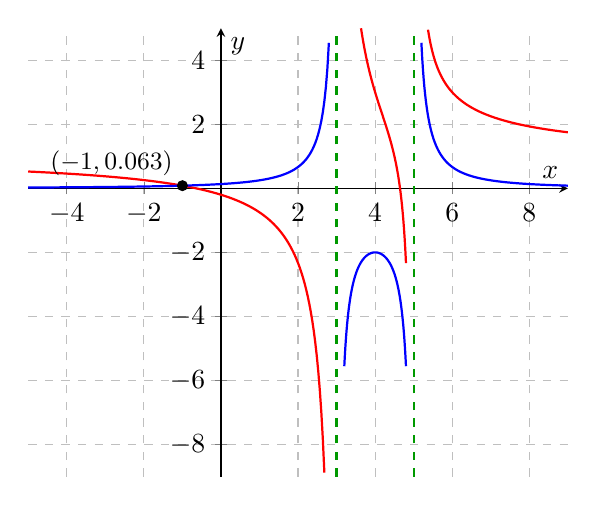
\begin{tikzpicture}
\begin{axis}[
    axis lines=middle,
    xmin=-5, xmax=9,
    ymin=-9, ymax=5,
    xtick={-4,-2,0,2,4,6,8},
    ytick={-8,-6,-4,-2,0,2,4},
    grid=both,
    grid style={dashed, gray!50},
    xlabel={$x$},
    ylabel={$y$},
    samples=200
]
\addplot[domain=-5:2.8, color=red, thick, restrict y to domain=-9:5] {1/(x-5) + x/(x-3)};
\addplot[domain=3.2:4.8, color=red, thick, restrict y to domain=-9:5] {1/(x-5) + x/(x-3)};
\addplot[domain=5.2:9, color=red, thick, restrict y to domain=-9:5] {1/(x-5) + x/(x-3)};

\addplot[domain=-5:2.8, color=blue, thick, restrict y to domain=-9:5] {2/((x-3)*(x-5))};
\addplot[domain=3.2:4.8, color=blue, thick, restrict y to domain=-9:5] {2/((x-3)*(x-5))};
\addplot[domain=5.2:9, color=blue, thick, restrict y to domain=-9:5] {2/((x-3)*(x-5))};

\draw[dashed, green!60!black, thick] (3,-9) -- (3,5);
\draw[dashed, green!60!black, thick] (5,-9) -- (5,5);

\fill[black] (-1, 0.083) circle (2pt);
\node[anchor=south east, font=\small] at (-1, 0.083) {$(-1, 0.063)$};
\end{axis}
\end{tikzpicture}
\end{center}

Both graphs have vertical asymptotes at $x = 3$ and $x = 5$. Therefore, neither graph has a value at $x = 5$. The graphs only intersect in one point, at $x = -1$.

\textit{CONCEPTUAL UNDERSTANDING: LOOK FOR RELATIONSHIPS How are an extraneous solution and an asymptote related? Is this always true?}
\end{example}

\begin{tryit}{3}
What is the solution to the equation $\frac{1}{x+2} + \frac{1}{x-2} = \frac{4}{(x+2)(x-2)}$?
\answer{\text{no solution}}
\end{tryit}

\begin{example}{4}
\textbf{Check for Extraneous Solutions}

What are the solutions to the following equations?

\textbf{A.} $\frac{5x}{x-2} = 7 + \frac{10}{x-2}$
\begin{align*}
\frac{5x}{x-2} &= 7 + \frac{10}{x-2} \\
(x-2)\left(\frac{5x}{x-2}\right) &= \left(7 + \frac{10}{x-2}\right)(x-2) \\
5x &= 7(x-2) + 10 \\
5x &= 7x - 14 + 10 \\
-2x &= -4 \\
x &= 2
\end{align*}
Check the solution in the original equation. The value 2 is an extraneous solution because it would cause the denominator in the original equation to be equal to 0.

This equation has no solution.

\textbf{B.} $\frac{3}{x-3} = \frac{x}{x-3} - \frac{x}{4}$
\begin{align*}
\frac{3}{x-3} &= \frac{x}{x-3} - \frac{x}{4} \\
(4)(x-3)\left(\frac{3}{x-3}\right) &= \left(\frac{x}{x-3} - \frac{x}{4}\right)(4)(x-3) \\
4(3) &= 4(x) - x(x-3) \\
12 &= 4x - x^2 + 3x \\
x^2 - 7x + 12 &= 0 \\
(x-3)(x-4) &= 0 \\
x - 3 = 0 &\text{ or } x - 4 = 0 \\
x = 3 &\text{ or } x = 4
\end{align*}
Check the solutions in the original equation. The value 3 is an extraneous solution because it would cause the denominator of the original equation to be equal to zero. The only solution to the equation is $x = 4$.

\textit{HAVE A GROWTH MINDSET: In what ways do you give your best effort and persist?}
\end{example}

\begin{tryit}{4}
What are the solutions to the following equations? \\
\textbf{a.} $x + \frac{6}{x-3} = \frac{2x}{x-3}$ \answer{x = 2} \\
\textbf{b.} $\frac{x^2}{x+5} = \frac{25}{x+5}$ \answer{x = 5}
\end{tryit}

\begin{example}{5}
\textbf{Solve a Rate Problem}

Paddling with the current in a river, Jake traveled 16 miles. Even though he paddled upstream for an hour longer than the amount of time he paddled downstream, Jake could only travel 6 miles against the current. In still water, Jake paddles at a rate of 5 mph. What is the speed of the current in the river?

\placeholder{illustration}{Jake paddling a canoe on a river. Arrows indicate "16 miles downstream" and "6 miles upstream".}

\textbf{Formulate} \quad Let $c$ be the rate of the river's current in miles per hour.
Recall that $\text{distance} = \text{rate} \cdot \text{time}$, so $\text{time} = \frac{\text{distance}}{\text{rate}}$.

\[
\frac{16}{\underbrace{5+c}_{\text{Jake's paddle rate in still water + the rate of the current}}} + \underbrace{1}_{\text{Jake paddles 1 h longer upstream than downstream.}} = \frac{6}{\underbrace{5-c}_{\text{Jake's paddle rate in still water - the rate of the current}}}
\]

\textbf{Compute} \quad Solve the equation for $c$.
\begin{align*}
\frac{16}{5+c} + 1 &= \frac{6}{5-c} \\
(5+c)(5-c)\left(\frac{16}{5+c} + 1\right) &= \left(\frac{6}{5-c}\right)(5+c)(5-c) \\
80 - 16c + 25 - c^2 &= 30 + 6c \\
0 &= c^2 + 22c - 75 \\
0 &= (c+25)(c-3) \\
0 = c + 25 &\quad 0 = c - 3 \\
c = -25 &\quad c = 3
\end{align*}

\textbf{Interpret} \quad The solution $c = -25$ is extraneous because the speed of the current cannot be negative.
The speed of the current is 3 mph.
\end{example}

\begin{tryit}{5}
Three people are planting tomatoes in a community garden. Marta takes 50 minutes to plant the garden alone, Benito takes $x$ minutes and Tyler takes $x + 15$ minutes. If the three of them take 20 minutes to finish the garden, how long would it have taken Tyler alone?
\answer{75 \text{ minutes}}
\end{tryit}

\begin{concept-summary}
\textbf{CONCEPT SUMMARY: Solving Rational Equations}

\textbf{WORDS}
A rational equation is an equation that contains a rational expression. To solve, identify the domain for the variable. Then multiply both sides of the equation by a common denominator and solve. An extraneous solution is a solution that is not valid because that value is excluded from the domain of the original equation.

\textbf{ALGEBRA}
\begin{align*}
\frac{1}{x} + \frac{2}{x} &= \frac{1}{6} \quad \text{Domain: } x \neq 0 \\
6x\left(\frac{1}{x} + \frac{2}{x}\right) &= 6x\left(\frac{1}{6}\right) \\
6 + 12 &= x \\
18 &= x
\end{align*}
The domain includes $x = 18$, so the solution to the equation is 18.

\begin{align*}
\frac{x^2+4}{x-1} &= \frac{5}{x-1} \quad \text{Domain: } x \neq 1 \\
(x-1)\left(\frac{x^2+4}{x-1}\right) &= (x-1)\left(\frac{5}{x-1}\right) \\
x^2+4 &= 5 \\
x^2 &= 1 \\
x &= \pm 1
\end{align*}
The domain does not include $x = 1$, so 1 is an extraneous solution. It does include $x = -1$, so the solution to the equation is $-1$.
\end{concept-summary}

\section*{Do You UNDERSTAND?}
\begin{practice}{1}{DOK}
\textbf{ESSENTIAL QUESTION} How can you solve rational equations and identify extraneous solutions?
\end{practice}

\begin{practice}{2}{DOK}
\textbf{Vocabulary} Write your own example of a rational equation that, when solved, has at least one \textbf{extraneous solution}.
\end{practice}

\begin{practice}{3}{DOK}
\textbf{Error Analysis} A student solved the rational equation as follows:
\[ \frac{1}{2x} - \frac{2}{5x} = \frac{1}{10x} - 3; \ x = 0 \]
Describe and correct the error the student made.
\answer{The student did not check for extraneous solutions. The value $x = 0$ is extraneous because it makes the denominators zero. Therefore, there is no solution.}
\end{practice}

\begin{practice}{4}{DOK}
\textbf{Construct Arguments} Yuki says, \textit{"You can check the solution(s) of rational equations in any of the steps of the solution process."} Explain why her reasoning is incorrect.
\end{practice}

\section*{Do You KNOW HOW?}
Solve.
\begin{practice}{5}{DOK}
$\frac{4}{x+6} = 2$
\answer{x = -4}
\end{practice}

\begin{practice}{6}{DOK}
$\frac{x^2}{x+3} = \frac{9}{x+3}$
\answer{x = -3 \text{ is an extraneous solution, so the only solution is } x = 3.}
\end{practice}

\begin{practice}{7}{DOK}
Organizing given information into a table can be helpful when solving rate problems. Use this table to solve the following problem.
\begin{center}
\begin{tabular}{|l|c|c|c|}
\hline
& \textbf{Distance} & \textbf{Rate} & \textbf{Time} \\
\hline
\textbf{Upstream} & & & \\
\hline
\textbf{Downstream} & & & \\
\hline
\end{tabular}
\end{center}
A boat can travel 6 km upstream in the same time it takes to travel 12 km downstream. Find the speed of the boat in still water.

\placeholder{illustration}{A boat on a river with labels River Current = 4 km/h, Upstream: 6 km, Downstream: 12 km}
\answer{Boat speed in still water is 12 km/h.}
\end{practice}

\section*{PRACTICE \& PROBLEM SOLVING}

\subsection*{UNDERSTAND}
\begin{practice}{8}{DOK}
\textbf{Reason} If you solve a work-rate problem and your solution, which represents the amount of time it would take \textit{working together}, exceeds the individual \textit{working alone} times that are given, then how do you know your solution is unreasonable? Explain.
\end{practice}

\begin{practice}{9}{DOK}
\textbf{Construct Arguments} Explain why a negative solution must be eliminated as an extraneous solution when solving a rational equation for an unknown rate.
\end{practice}

\begin{practice}{10}{DOK}
\textbf{Error Analysis} Describe and correct the error Miranda made in solving the rational equation.
\begin{align*}
\frac{1}{x-2} + \frac{x-2}{x+2} &= \frac{x-4}{x-2} \\
(x+2)(x-2)\left(\frac{1}{x-2} + \frac{x-2}{x+2}\right) &= \left(\frac{x-4}{x-2}\right)(x+2)(x-2) \\
(x+2)(1) + (x-2)(x-2) &= (x+4)(x+2) \\
x + 2 + x^2 - 4x + 4 &= x^2 + 6x + 8 \\
-3x + 6 &= 6x + 8 \\
-2 &= 9x; \text{ or } x = -\frac{2}{9} \quad \text{\textbf{X}}
\end{align*}
\answer{Miranda incorrectly expanded the right side as $(x+4)(x+2)$ instead of $(x-4)(x+2)$. The correct right side is $x^2 - 2x - 8$. Solving $-3x + 6 = -2x - 8$ yields $x = 14$.}
\end{practice}

\begin{practice}{11}{DOK}
\textbf{Generalize} In addition to identifying extraneous solutions, why else is it important to substitute your solution into the original equation?
\answer{To check for algebraic and arithmetic errors in the solving process.}
\end{practice}

\begin{practice}{12}{DOK}
\textbf{Mathematical Connections} Explain how solving rational equations is related to solving linear and quadratic equations.
\answer{Multiplying a rational equation by the least common denominator transforms it into a polynomial equation, typically linear or quadratic, which can then be solved using standard methods.}
\end{practice}

\begin{practice}{13}{DOK}
\textbf{Higher Order Thinking} Write a rational equation that cannot have 2 or $-6$ as solutions.
\answer{\text{Sample answer: } \frac{1}{x-2} + \frac{1}{x+6} = 0}
\end{practice}

\begin{practice}{14}{DOK}
\textbf{Make Sense and Persevere} Solve the rational equation shown. Explain what is unique about the solution.
\[ \frac{x^2 - 7x - 18}{x+2} = x - 9 \]
\answer{The solution is all real numbers except $x = -2$. Factoring the numerator shows that the equation is an identity $\frac{(x-9)(x+2)}{x+2} = x-9$, which is true for all $x$ in the domain.}
\end{practice}

\subsection*{PRACTICE}
Solve the equation. SEE EXAMPLE 1
\begin{practice}{15}{DOK}
$\frac{1}{x-3} = 10$
\answer{x = 3.1 \text{ or } \frac{31}{10}}
\end{practice}

\begin{practice}{16}{DOK}
$\frac{15}{x+3} = 3$
\answer{x = 2}
\end{practice}

\begin{practice}{17}{DOK}
$\frac{12}{x-4} = 9$
\answer{x = \frac{16}{3}}
\end{practice}

\begin{practice}{18}{DOK}
$\frac{5}{3-x} = 1$
\answer{x = -2}
\end{practice}

Solve the problem. SEE EXAMPLE 2
\begin{practice}{19}{DOK}
Working individually, Paige and Malia can each complete a landscaping job in the time shown. Working together, how long would it take them to complete the job?
\placeholder{illustration}{Malia and Paige landscaping. Labels: Malia 4 hours, Paige 6 hours}
\answer{2.4 \text{ hours}}
\end{practice}

\begin{practice}{20}{DOK}
Russel and Aaron can build a shed in the time shown when working together. Aaron works three times as fast as Russel. How long would it take Russel to build the shed if he were to work alone?
\placeholder{illustration}{Russel and Aaron building a shed. Label: Russel and Aaron can build the shed in 8 hours working together.}
\answer{32 \text{ hours}}
\end{practice}

Solve the equation. SEE EXAMPLE 3
\begin{practice}{21}{DOK}
$\frac{x}{x-3} - 4 = \frac{3}{x-3}$
\answer{\text{no solution}}
\end{practice}

\begin{practice}{22}{DOK}
$\frac{x^2}{x-10} = \frac{100}{x-10} - 10$
\answer{x = -20}
\end{practice}

Solve the equation. SEE EXAMPLE 4
\begin{practice}{23}{DOK}
$\frac{4}{3(x+1)} = \frac{12}{x^2-1}$
\answer{x = 10}
\end{practice}

\begin{practice}{24}{DOK}
$\frac{x}{x-3} + \frac{2x}{x+3} = \frac{18}{(x+3)(x-3)}$
\answer{x = -2}
\end{practice}

Solve the problem. SEE EXAMPLE 5
\begin{practice}{25}{DOK}
A boat travels 8 miles upstream in the same amount of time it can travel 12 miles downstream. In still water the speed of the boat is 5 mi/h. What is the speed of the current?
\answer{1 \text{ mi/h}}
\end{practice}

\subsection*{APPLY}
\begin{practice}{25}{DOK}
\textbf{Make Sense and Persevere} Kenji can finish a puzzle in 2 hours working alone. Oscar can finish the same puzzle in 3 hours working alone. How long would it take Oscar and Kenji to finish the puzzle if they worked on it together?
\answer{1.2 \text{ hours}}
\end{practice}

\begin{practice}{26}{DOK}
\textbf{Use Structure} A commercial jet flies 1,500 miles with the wind. In the same amount of time it can fly 1,000 miles against the wind. The speed of the jet in still air is 550 mph. Find the speed of the wind.
\placeholder{illustration}{A commercial jet flying with an arrow indicating "Wind Direction" and another pointing backwards labeled "1,000 miles".} \\
\textbf{a.} Organize the given information and what you need to find in a table. \\
\textbf{b.} Write and solve a rational equation to find the wind speed.
\answer{
\textbf{a.} 
\begin{tabular}{|l|c|c|c|}
\hline
& Distance & Rate & Time \\
\hline
With wind & 1500 & 550+w & 1500/(550+w) \\
Against wind & 1000 & 550-w & 1000/(550-w) \\
\hline
\end{tabular} \\
\textbf{b.} $\frac{1500}{550+w} = \frac{1000}{550-w}; w = 110 \text{ mph}$
}
\end{practice}

\begin{practice}{27}{DOK}
\textbf{Reason} During their day at the beach, Jae and his friends rent a Jet Ski. They split the \$120 rental fee evenly among themselves. Then Jae, with only his friend Orion, share the cost of a \$16 pizza. If Jae spends a total of \$48 for both, then find the number of friends, $n$, with whom he shared the cost of the Jet Ski rental.
\answer{n = 3}
\end{practice}

\begin{practice}{28}{DOK}
\textbf{Make Sense and Persevere} When driving to their family reunion, Rio's mom drove 10 miles at a rate of $x$ mph and then 25 miles at a rate of $x + 10$ mph. The total driving time was 45 minutes. What were the two driving speeds at which Rio's mom drove?
\answer{40 \text{ mph and } 50 \text{ mph}}
\end{practice}

\begin{practice}{29}{DOK}
\textbf{Generalize} So far this baseball season, Philip has gotten a hit 8 times out of 40 at-bats. He wants to increase his batting average to 0.333. Calculate the number of consecutive hits, $h$, he would need in order to achieve this goal. Round your answer to the nearest whole number.
\answer{h = 8}
\end{practice}

\subsection*{ASSESSMENT PRACTICE}
\begin{practice}{30}{DOK}
Which of the following rational equations have at least one extraneous solution? Select all that apply. \\
$\square \ \frac{2}{x} = \frac{3}{x-4}$ \\
$\square \ \frac{x^2}{x-3} = \frac{9}{x-3}$ \\
$\square \ \frac{x-1}{x-5} = \frac{9}{x-5}$ \\
$\square \ x + \frac{3}{x} = 4$ \\
$\square \ \frac{x}{x-3} - \frac{3}{2} = \frac{3}{x-3}$
\answer{$\frac{x^2}{x-3} = \frac{9}{x-3}$ and $\frac{x}{x-3} - \frac{3}{2} = \frac{3}{x-3}$}
\end{practice}

\begin{practice}{31}{DOK}
\textbf{SAT/ACT} Which of the following is the solution of $\frac{3}{x+1} = \frac{2}{x-3}$? \\
\textcircled{A} \ $x = -11$ \\
\textcircled{B} \ $x = -\frac{7}{5}$ \\
\textcircled{C} \ $x = \frac{7}{5}$ \\
\textcircled{D} \ $x = 11$
\answer{D}
\end{practice}

\begin{practice}{32}{DOK}
\textbf{Performance Task} A chemist needs alcohol solution in the correct concentration for her experiment. She adds a 6\% alcohol solution to 50 gallons of solution that is 2\% alcohol. The function that represents the percent of alcohol in the resulting solution is $f(x) = \frac{50(0.02) + x(0.06)}{50 + x}$, where $x$ is the amount of 6\% solution added.

\placeholder{illustration}{A chemist pouring liquid from a beaker into a larger container. Labels: "$x$ gallons of 6\% alcohol" and "50 gallons of 2\% alcohol".}

\textbf{Part A} How much 6\% solution should be added to create a solution that is 5\% alcohol? \\
\textbf{Part B Use Appropriate Tools} Explain the steps you could take to use your graphing calculator to verify the correctness of your answer to part (A).
\answer{
\textbf{Part A} 150 gallons \\
\textbf{Part B} Graph the equations $Y_1 = \frac{1 + 0.06X}{50 + X}$ and $Y_2 = 0.05$. Use the calculator's intersection feature to find the coordinates where the graphs cross. The $X$-coordinate of the intersection is 150, which verifies the solution.
}
\end{practice}

\end{document}